\documentclass{standalone}
\usepackage{tikz}
\usetikzlibrary{patterns, positioning}


\begin{document}
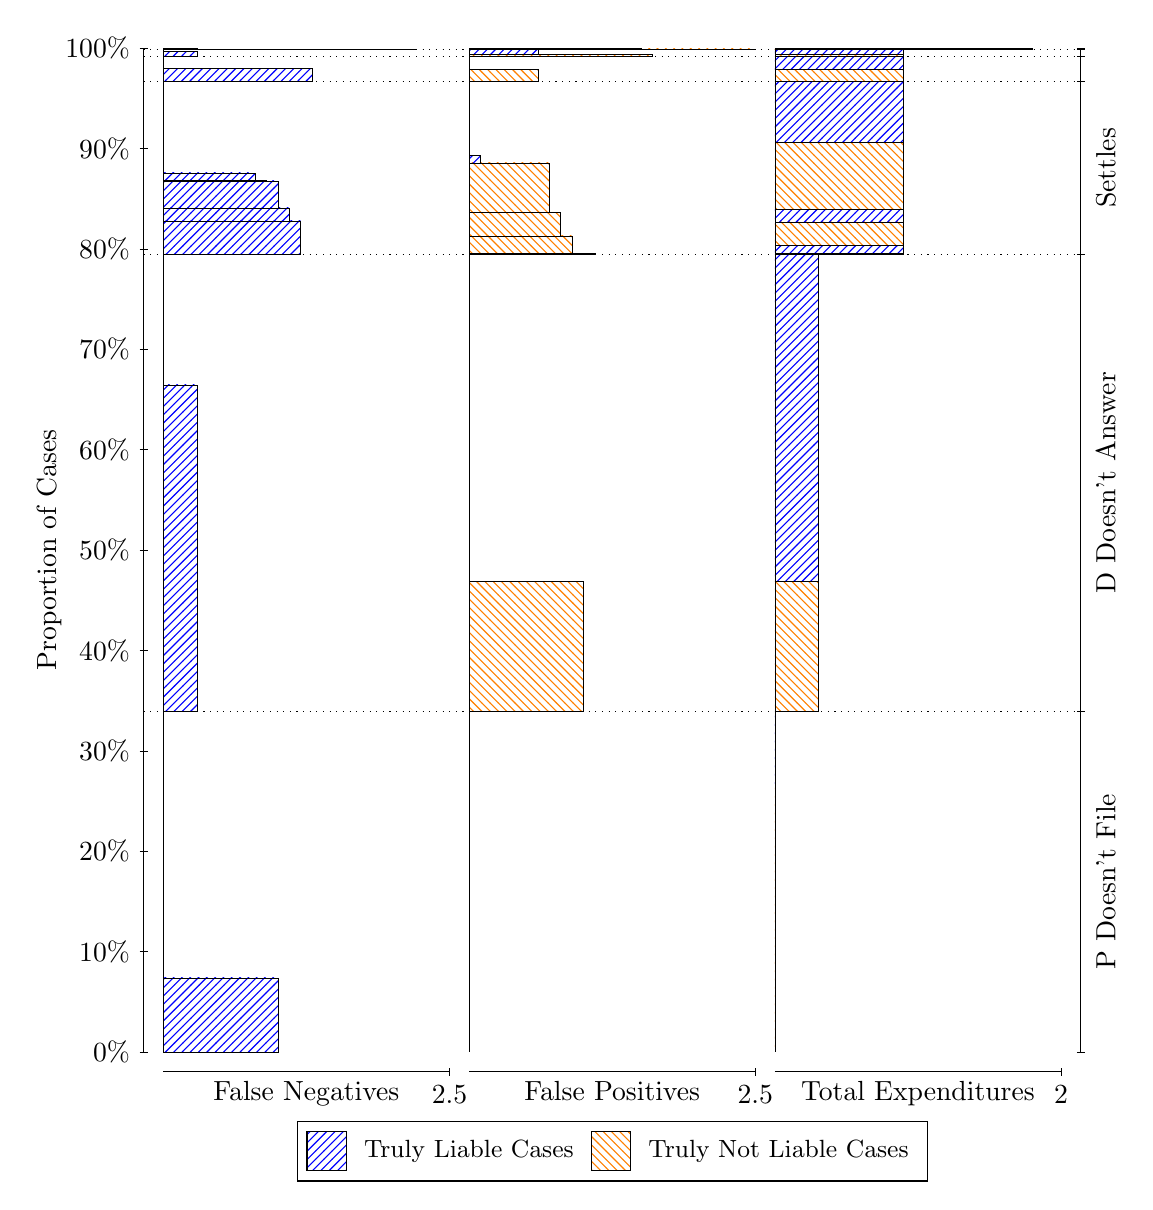
\begin{tikzpicture}
\draw[black, very thin] (1.5,1.75) -- (1.5,14.5);
\node[rotate=90, text=black, anchor=center] at (0.3, 8.125) {Proportion of Cases};
\draw[black, very thin] (1.45,1.75) -- (1.55,1.75);
\node[text=black, anchor=east] at (1.45, 1.75) {0\%};
\draw[black, very thin] (1.45,3.025) -- (1.55,3.025);
\node[text=black, anchor=east] at (1.45, 3.025) {10\%};
\draw[black, very thin] (1.45,4.3) -- (1.55,4.3);
\node[text=black, anchor=east] at (1.45, 4.3) {20\%};
\draw[black, very thin] (1.45,5.575) -- (1.55,5.575);
\node[text=black, anchor=east] at (1.45, 5.575) {30\%};
\draw[black, very thin] (1.45,6.85) -- (1.55,6.85);
\node[text=black, anchor=east] at (1.45, 6.85) {40\%};
\draw[black, very thin] (1.45,8.125) -- (1.55,8.125);
\node[text=black, anchor=east] at (1.45, 8.125) {50\%};
\draw[black, very thin] (1.45,9.4) -- (1.55,9.4);
\node[text=black, anchor=east] at (1.45, 9.4) {60\%};
\draw[black, very thin] (1.45,10.675) -- (1.55,10.675);
\node[text=black, anchor=east] at (1.45, 10.675) {70\%};
\draw[black, very thin] (1.45,11.95) -- (1.55,11.95);
\node[text=black, anchor=east] at (1.45, 11.95) {80\%};
\draw[black, very thin] (1.45,13.225) -- (1.55,13.225);
\node[text=black, anchor=east] at (1.45, 13.225) {90\%};
\draw[black, very thin] (1.45,14.5) -- (1.55,14.5);
\node[text=black, anchor=east] at (1.45, 14.5) {100\%};

\draw[black, very thin] (13.4,1.75) -- (13.4,14.5);
\draw[black, very thin] (13.35,1.75) -- (13.45,1.75);
\node[anchor=west] at (13.35, 1.75) {};
\draw[black, very thin] (13.35,6.0707) -- (13.45,6.0707);
\node[anchor=west] at (13.35, 6.0707) {};
\draw[black, very thin] (13.35,11.882) -- (13.45,11.882);
\node[anchor=west] at (13.35, 11.882) {};
\draw[black, very thin] (13.35,14.074) -- (13.45,14.074);
\node[anchor=west] at (13.35, 14.074) {};
\draw[black, very thin] (13.35,14.397) -- (13.45,14.397);
\node[anchor=west] at (13.35, 14.397) {};
\draw[black, very thin] (13.35,14.48) -- (13.45,14.48);
\node[anchor=west] at (13.35, 14.48) {};
\draw[black, very thin] (13.35,14.486) -- (13.45,14.486);
\node[anchor=west] at (13.35, 14.486) {};
\draw[black, very thin] (13.35,14.5) -- (13.45,14.5);
\node[anchor=west] at (13.35, 14.5) {};

\draw[black, very thin, pattern color=blue, pattern=north east lines] (1.75,1.75) rectangle (3.2033,2.6909);
\draw[black, very thin, pattern color=orange, pattern=north west lines] (1.75,2.6909) rectangle (1.75,6.0707);
\draw[black, very thin, pattern color=blue, pattern=north east lines] (1.75,6.0707) rectangle (2.186,10.223);
\draw[black, very thin, pattern color=orange, pattern=north west lines] (1.75,10.223) rectangle (1.75,11.882);
\draw[black, very thin, pattern color=blue, pattern=north east lines] (1.75,11.882) rectangle (3.494,12.306);
\draw[black, very thin, pattern color=blue, pattern=north east lines] (1.75,12.306) rectangle (3.3487,12.469);
\draw[black, very thin, pattern color=blue, pattern=north east lines] (1.75,12.469) rectangle (3.2033,12.812);
\draw[black, very thin, pattern color=blue, pattern=north east lines] (1.75,12.812) rectangle (3.058,12.816);
\draw[black, very thin, pattern color=blue, pattern=north east lines] (1.75,12.816) rectangle (2.9127,12.915);
\draw[black, very thin, pattern color=orange, pattern=north west lines] (1.75,12.915) rectangle (1.75,14.074);
\draw[black, very thin, pattern color=blue, pattern=north east lines] (1.75,14.074) rectangle (3.6393,14.245);
\draw[black, very thin, pattern color=orange, pattern=north west lines] (1.75,14.245) rectangle (1.75,14.397);
\draw[black, very thin, pattern color=blue, pattern=north east lines] (1.75,14.397) rectangle (2.186,14.462);
\draw[black, very thin, pattern color=orange, pattern=north west lines] (1.75,14.462) rectangle (1.75,14.48);
\draw[black, very thin, pattern color=blue, pattern=north east lines] (1.75,14.48) rectangle (4.9473,14.483);
\draw[black, very thin, pattern color=orange, pattern=north west lines] (1.75,14.483) rectangle (1.75,14.486);
\draw[black, very thin, pattern color=blue, pattern=north east lines] (1.75,14.486) rectangle (2.186,14.497);
\draw[black, very thin, pattern color=orange, pattern=north west lines] (1.75,14.497) rectangle (1.75,14.5);
\draw[black, very thin, pattern color=orange, pattern=north west lines] (5.6333,1.75) rectangle (5.6333,5.1298);
\draw[black, very thin, pattern color=blue, pattern=north east lines] (5.6333,5.1298) rectangle (5.6333,6.0707);
\draw[black, very thin, pattern color=orange, pattern=north west lines] (5.6333,6.0707) rectangle (7.0867,7.7303);
\draw[black, very thin, pattern color=blue, pattern=north east lines] (5.6333,7.7303) rectangle (5.6333,11.882);
\draw[black, very thin, pattern color=orange, pattern=north west lines] (5.6333,11.882) rectangle (7.232,11.894);
\draw[black, very thin, pattern color=orange, pattern=north west lines] (5.6333,11.894) rectangle (7.0867,11.896);
\draw[black, very thin, pattern color=orange, pattern=north west lines] (5.6333,11.896) rectangle (6.9413,12.114);
\draw[black, very thin, pattern color=orange, pattern=north west lines] (5.6333,12.114) rectangle (6.796,12.413);
\draw[black, very thin, pattern color=orange, pattern=north west lines] (5.6333,12.413) rectangle (6.6507,13.042);
\draw[black, very thin, pattern color=blue, pattern=north east lines] (5.6333,13.042) rectangle (5.7787,13.141);
\draw[black, very thin, pattern color=blue, pattern=north east lines] (5.6333,13.141) rectangle (5.6333,14.074);
\draw[black, very thin, pattern color=orange, pattern=north west lines] (5.6333,14.074) rectangle (6.5053,14.226);
\draw[black, very thin, pattern color=blue, pattern=north east lines] (5.6333,14.226) rectangle (5.6333,14.397);
\draw[black, very thin, pattern color=orange, pattern=north west lines] (5.6333,14.397) rectangle (7.9587,14.415);
\draw[black, very thin, pattern color=blue, pattern=north east lines] (5.6333,14.415) rectangle (6.5053,14.48);
\draw[black, very thin, pattern color=orange, pattern=north west lines] (5.6333,14.48) rectangle (6.5053,14.483);
\draw[black, very thin, pattern color=blue, pattern=north east lines] (5.6333,14.483) rectangle (5.6333,14.486);
\draw[black, very thin, pattern color=orange, pattern=north west lines] (5.6333,14.486) rectangle (9.2667,14.489);
\draw[black, very thin, pattern color=blue, pattern=north east lines] (5.6333,14.489) rectangle (7.8133,14.5);
\draw[black, very thin, pattern color=orange, pattern=north west lines] (9.5167,1.75) rectangle (9.5167,5.1298);
\draw[black, very thin, pattern color=blue, pattern=north east lines] (9.5167,5.1298) rectangle (9.5167,6.0707);
\draw[black, very thin, pattern color=orange, pattern=north west lines] (9.5167,6.0707) rectangle (10.062,7.7303);
\draw[black, very thin, pattern color=blue, pattern=north east lines] (9.5167,7.7303) rectangle (10.062,11.882);
\draw[black, very thin, pattern color=orange, pattern=north west lines] (9.5167,11.882) rectangle (11.152,11.894);
\draw[black, very thin, pattern color=blue, pattern=north east lines] (9.5167,11.894) rectangle (11.152,11.993);
\draw[black, very thin, pattern color=orange, pattern=north west lines] (9.5167,11.993) rectangle (11.152,12.293);
\draw[black, very thin, pattern color=blue, pattern=north east lines] (9.5167,12.293) rectangle (11.152,12.455);
\draw[black, very thin, pattern color=orange, pattern=north west lines] (9.5167,12.455) rectangle (11.152,13.304);
\draw[black, very thin, pattern color=blue, pattern=north east lines] (9.5167,13.304) rectangle (11.152,14.074);
\draw[black, very thin, pattern color=orange, pattern=north west lines] (9.5167,14.074) rectangle (11.152,14.226);
\draw[black, very thin, pattern color=blue, pattern=north east lines] (9.5167,14.226) rectangle (11.152,14.397);
\draw[black, very thin, pattern color=orange, pattern=north west lines] (9.5167,14.397) rectangle (11.152,14.415);
\draw[black, very thin, pattern color=blue, pattern=north east lines] (9.5167,14.415) rectangle (11.152,14.48);
\draw[black, very thin, pattern color=orange, pattern=north west lines] (9.5167,14.48) rectangle (12.787,14.483);
\draw[black, very thin, pattern color=blue, pattern=north east lines] (9.5167,14.483) rectangle (12.787,14.486);
\draw[black, very thin, pattern color=orange, pattern=north west lines] (9.5167,14.486) rectangle (12.787,14.489);
\draw[black, very thin, pattern color=blue, pattern=north east lines] (9.5167,14.489) rectangle (12.787,14.5);
\draw[black, dotted] (1.5,6.0707) -- (13.4,6.0707);
\draw[black, dotted] (1.5,11.882) -- (13.4,11.882);
\draw[black, dotted] (1.5,14.074) -- (13.4,14.074);
\draw[black, dotted] (1.5,14.397) -- (13.4,14.397);
\draw[black, dotted] (1.5,14.48) -- (13.4,14.48);
\draw[black, dotted] (1.5,14.486) -- (13.4,14.486);
\draw[black, very thin] (1.75,1.5) -- (5.3833,1.5);
\node[text=black, anchor=north] at (3.5667, 1.5) {False Negatives};
\draw[black, very thin] (5.3833,1.45) -- (5.3833,1.55);
\node[text=black, anchor=north] at (5.3833, 1.45) {2.5};

\draw[black, very thin] (5.6333,1.5) -- (9.2667,1.5);
\node[text=black, anchor=north] at (7.45, 1.5) {False Positives};
\draw[black, very thin] (9.2667,1.45) -- (9.2667,1.55);
\node[text=black, anchor=north] at (9.2667, 1.45) {2.5};

\draw[black, very thin] (9.5167,1.5) -- (13.15,1.5);
\node[text=black, anchor=north] at (11.333, 1.5) {Total Expenditures};
\draw[black, very thin] (13.15,1.45) -- (13.15,1.55);
\node[text=black, anchor=north] at (13.15, 1.45) {2};

\node[text=black, centered, rotate=90] at (13.72, 3.9104) {P Doesn't File};
\node[text=black, centered, rotate=90] at (13.72, 8.9765) {D Doesn't Answer};
\node[text=black, centered, rotate=90] at (13.72, 12.978) {Settles};





\draw (7.449999999999999,1.5) node[draw=none] (baseCoordinate) {};
\begin{scope}[align=center]
        \matrix[scale=0.5, draw=black, below=0.5cm of baseCoordinate, nodes={draw}, column sep=0.1cm]{
            \node[rectangle, draw, minimum width=0.5cm, minimum height=0.5cm, pattern color=blue, pattern=north east lines] {}; &
            \node[draw=none, font=\small, text=black] (B) {Truly Liable Cases}; &
            \node[rectangle, draw, minimum width=0.5cm, minimum height=0.5cm, pattern color=orange, pattern=north west lines] {}; &
            \node[draw=none, font=\small, text=black] (B) {Truly Not Liable Cases}; \\
            };
\end{scope}

\end{tikzpicture}
\end{document}